El resultado mas prometedor no es una clasificacion final de planetas, sino la identificacion de grafos y regiones candidatos para inspeccion cientifica. En esta corrida, el espacio orbital PCA es prioritario porque combina estructura no trivial con baja dependencia de imputacion. El espacio termico es topologicamente complejo, pero debe tratarse con cautela por su alta fraccion de imputacion. La inclusion de densidad derivada reduce ligeramente la complejidad de Mapper, lo que sugiere que \texttt{pl\_dens} actua como coordenada regularizadora mas que como fuente independiente de nueva ramificacion.

\begin{figure}[H]
\centering
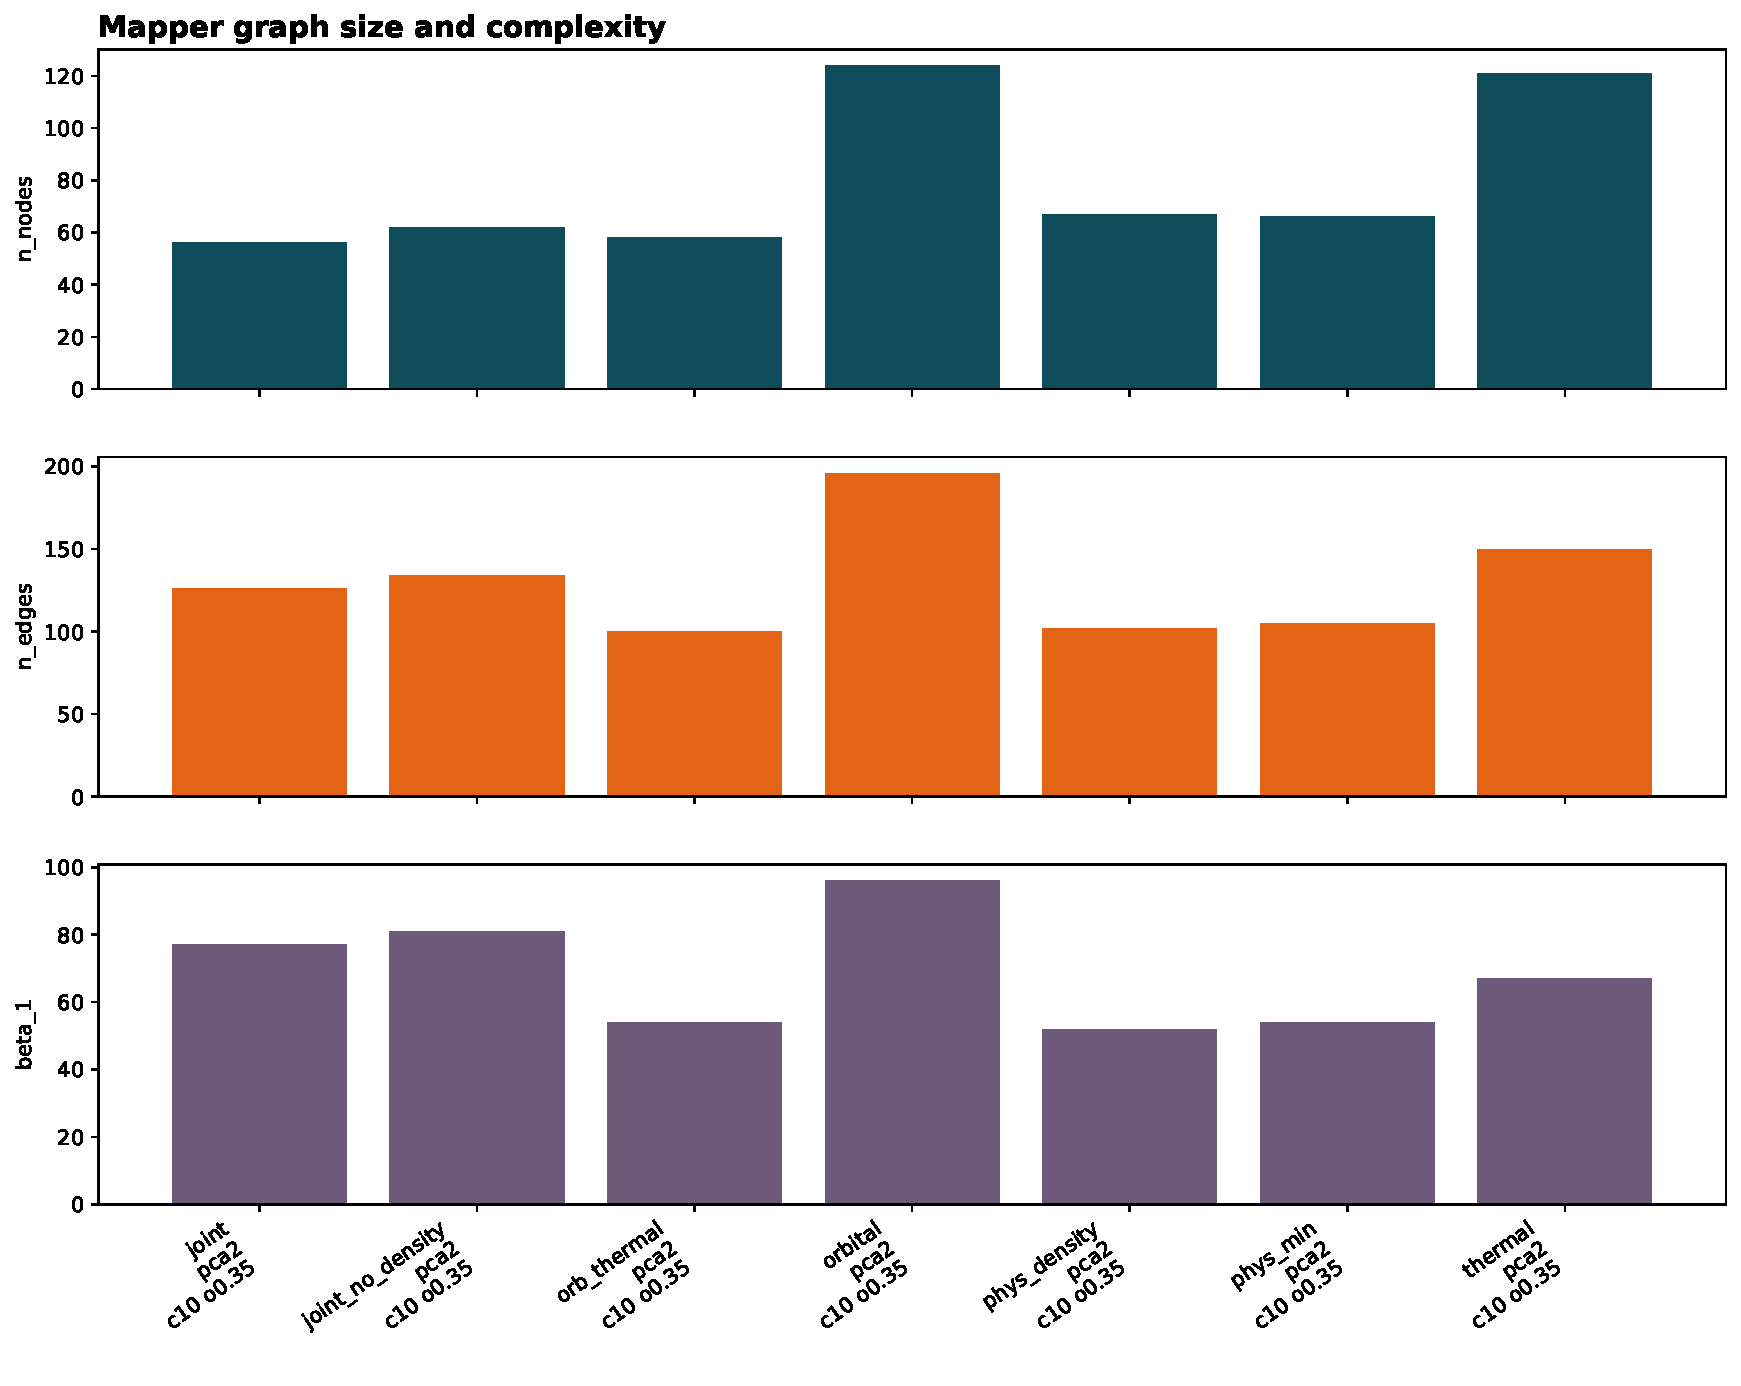
\includegraphics[width=0.95\linewidth]{figures/01_mapper_graph_size_complexity.pdf}
\caption{Tamano y complejidad de los grafos Mapper.}
\end{figure}

La Figura 1 resume el contraste estructural mas importante del reporte. El espacio orbital produce simultaneamente el mayor numero de nodos, el mayor numero de aristas y el mayor $\beta_1$, por lo que es el grafo con evidencia mas clara de ramificacion y ciclos. En cambio, los espacios fisicos y conjuntos quedan en una banda intermedia de complejidad. El espacio termico tambien aparece grande, pero no supera al orbital en ciclos, lo cual ya anticipa que su interes topologico debe evaluarse junto con la calidad de los datos y no solo con el tamano del grafo.

\begin{figure}[H]
\centering
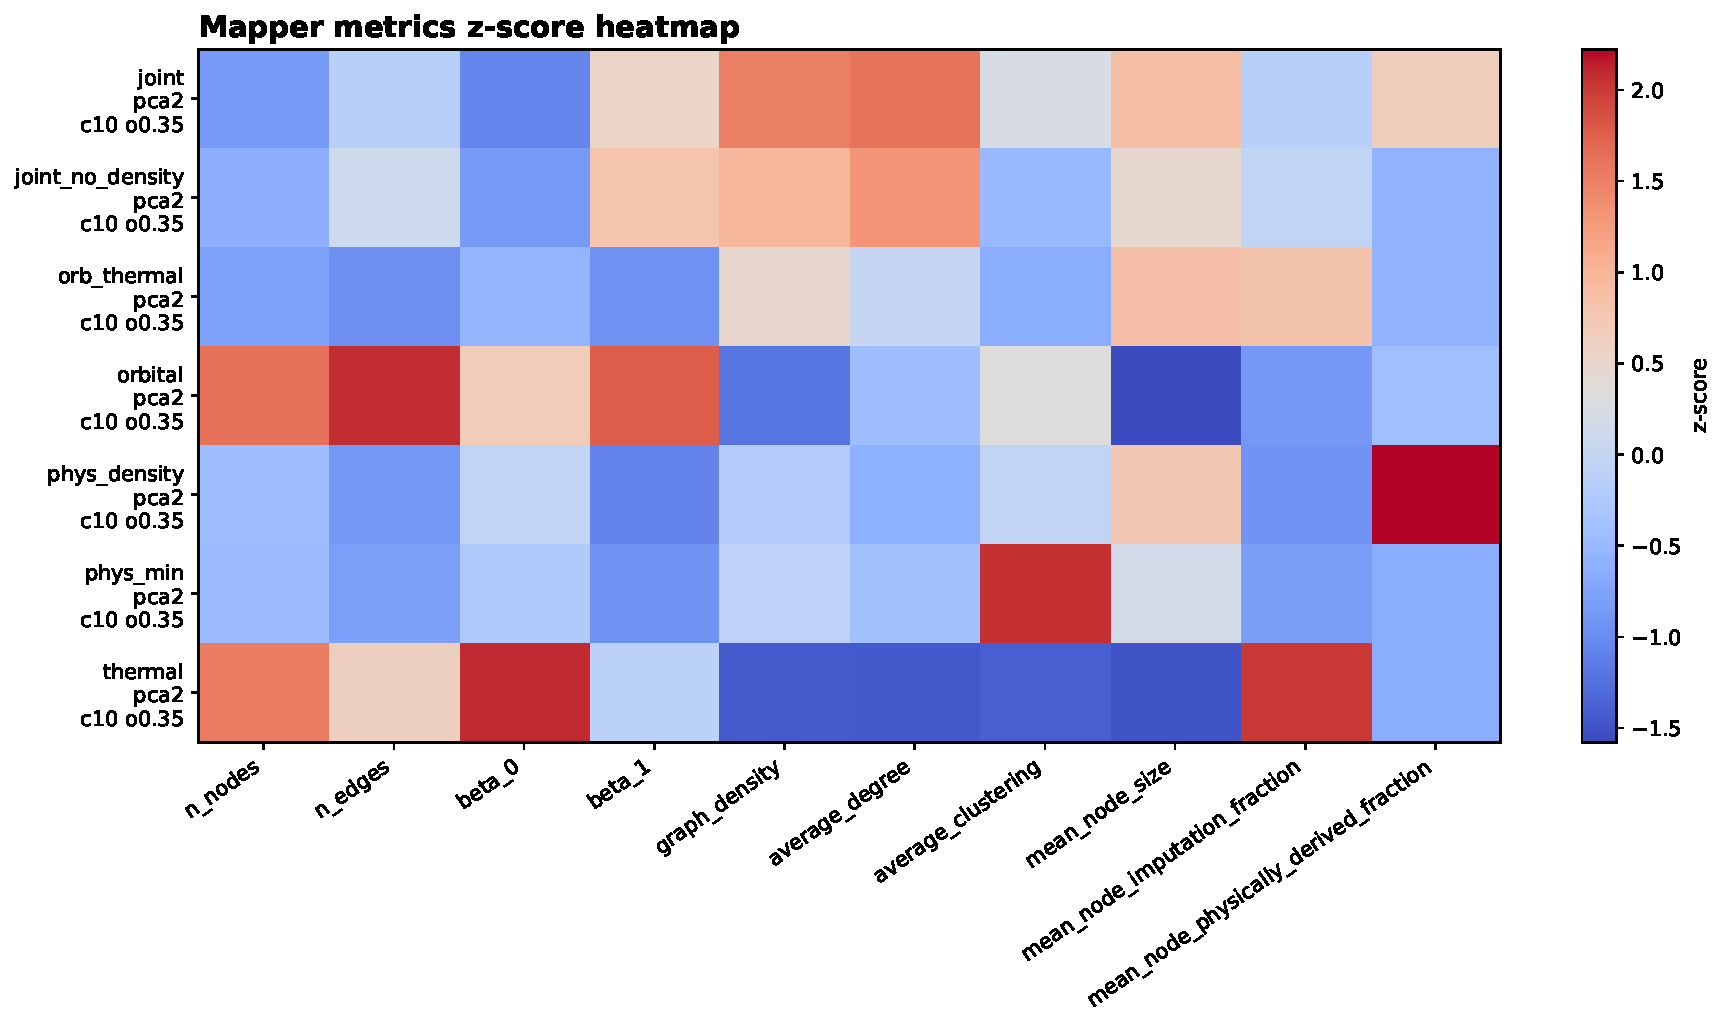
\includegraphics[width=0.95\linewidth]{figures/02_mapper_metrics_zscore_heatmap.pdf}
\caption{Heatmap de metricas estandarizadas.}
\end{figure}

La Figura 2 permite leer cada configuracion como un perfil relativo y no solo como un valor absoluto. La fila orbital destaca por sus z-scores altos en nodos, aristas y $\beta_1$, mientras que conserva una carga de imputacion baja. La fila termica muestra el patron opuesto: complejidad apreciable, pero acompanada por el z-score mas alto de imputacion. Las configuraciones con densidad derivada se separan por su mayor fraccion de variables fisicamente derivadas, lo cual es consistente con que \texttt{pl\_dens} agrega estructura algebraica mas que informacion observacional independiente.

\begin{figure}[H]
\centering
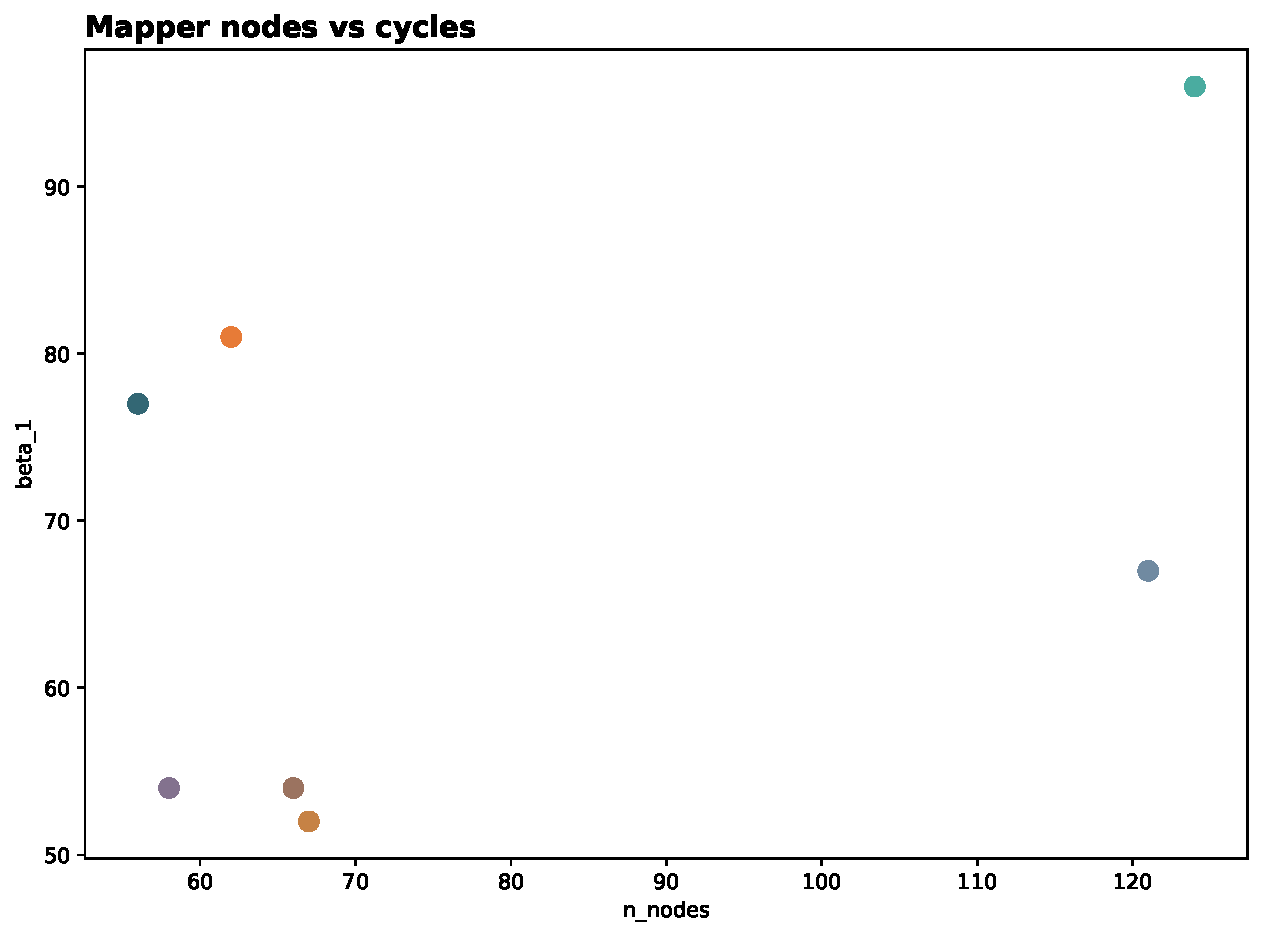
\includegraphics[width=0.75\linewidth]{figures/04_mapper_nodes_vs_cycles.pdf}
\caption{Relacion entre numero de nodos y ciclos.}
\end{figure}

La Figura 3 es util porque muestra que mas nodos no implican automaticamente mas interpretabilidad. Hay una tendencia positiva entre tamano del grafo y numero de ciclos, pero no todas las configuraciones con muchos nodos son igual de confiables. El caso orbital cae en la zona de alta complejidad con baja imputacion, mientras que el caso termico ocupa una zona parecida en escala pero con una lectura cientifica mas fragil. Por eso el reporte prioriza al espacio orbital aunque el termico tambien parezca visualmente rico.
